\documentclass[11pt]{amsart}

% margin stuff
\setlength{\textwidth}{6.25in}
\setlength{\oddsidemargin}{0in}
\setlength{\evensidemargin}{0in}
\setlength{\textheight}{8.5in}
\setlength{\topmargin}{-.25in}


\usepackage{amsthm,amsmath}
\theoremstyle{plain}
\newtheorem{prop}{Proposition}[section]
\newtheorem{puzzle}[prop]{Puzzle}
\newtheorem{conj}[prop]{Conjecture}
\newtheorem{thm}[prop]{Theorem}
\newtheorem{lem}[prop]{Lemma}

\usepackage{graphicx}
\newcommand{\mathfig}[2]{{\hspace{-3pt}\begin{array}{c}%
  \raisebox{-2.5pt}{\includegraphics[width=#1\textwidth]{#2}}%
\end{array}\hspace{-3pt}}}


\usepackage{tikz}
\usetikzlibrary{shapes}

\newcommand{\selfarrow}{\ensuremath{\smash{\tikz[baseline]{\clip (0,0.36) rectangle (0.48,-0.16); \draw[->] (0,0.175) .. controls (0.6,0.65) and (0.6,-0.45) .. (0,0.025);}}}}

\usepackage{hyperref}
\newcommand{\arxiv}[1]{\href{http://arxiv.org/abs/#1}{\tt arXiv:\nolinkurl{#1}}}

\newcommand{\bdy}{\partial}
\newcommand{\iso}{\cong}
\newcommand{\tensor}{\otimes}
\newcommand{\Tensor}{\bigotimes}

\newcommand{\into}{\hookrightarrow}

\newcommand{\restrict}[2]{#1{}_{\mid #2}{}}
\newcommand{\set}[1]{\left\{#1\right\}}
\newcommand{\setc}[2]{\setcl{#1}{#2}}

% tricky way to iterate macros over a list
\def\semicolon{;}
\def\applytolist#1{
    \expandafter\def\csname multi#1\endcsname##1{
        \def\multiack{##1}\ifx\multiack\semicolon
            \def\next{\relax}
        \else
            \csname #1\endcsname{##1}
            \def\next{\csname multi#1\endcsname}
        \fi
        \next}
    \csname multi#1\endcsname}

% \def\cA{{\cal A}} for A..Z
\def\calc#1{\expandafter\def\csname c#1\endcsname{{\mathcal #1}}}
\applytolist{calc}QWERTYUIOPLKJHGFDSAZXCVBNM;
\newcommand{\cl}[1]{\underrightarrow{#1}}

% \DeclareMathOperator{\pr}{pr} etc.
\def\declaremathop#1{\expandafter\DeclareMathOperator\csname #1\endcsname{#1}}
\applytolist{declaremathop}{Maps}{Diff}{Homeo}{Hom}{Cone};

\title{Fields and local relations}
\author{Scott Morrison \\ Notes for Teichner's hot topics course}
\date{January 25 2011}

\begin{document}
\maketitle

This talk is essentially a `warm-up' for the main ideas of the blob complex paper. For the most part, it's intended as a summary of how to think about topological quantum field theories via `fields and local relations'. We'll look at some examples of fields, and then use these to motivate the axiomatics. This will get us ready for reading \S 3, the first definition of the blob complex. As we go, I'll also sketch the relationship between fields and local relations and higher categories. For the most part I'll be a little vague about the definitions of higher categories, and instead try to talk about fields and local relations in a way that conveys the intuitions for our later definition of a `disklike $n$-category', in \S 6.

\section{Examples of fields}
The barebones data of an `$n$-dimensional system of fields' $\cF$ is a collection of functors $\cF_k$, for $0 \leq k \leq n$, from the groupoid of $k$-manifolds and homeomorphisms to the category of sets. That is, we have to specify the `set of fields on $M$', for any manifold $M$ of dimension at most $n$, along with a prescription for how these sets transform under homeomorphisms of $M$.

Whenever we have a system of fields, we also need the `local relations'. This is a functor $\cU$ from the groupoid of $n$-balls and homeomorphisms to the category of sets, such that $\cU \subset \cF$ and homeomorphisms act compatibly. Note that the local relations are only defined on balls, not arbitrary $n$-manifolds (hence `local'), and they only live at the top dimension.

There are two main examples which will motivate the precise definitions, so we'll go and understand these in some detail first.

\subsection{Maps to a target space}
Fixing a target space $T$, we can define a system of fields $\Maps(- \to T)$. Actually, it's best to modify this a bit, just in the top dimension, where we'll linearize in the following way: define $\Maps(X^n \to T)$ on an $n$-manifold $X$ to be \emph{formal linear combinations} of maps to $T$, extending a \emph{fixed} linear map on $\bdy X$. (That is, arbitrary boundary conditions are allowed, but we can only take linear combinations of maps with the same boundary conditions.) This will be a common feature for all `linear' systems of fields: at the top dimension the set associated to an $n$-manifold will break up into a vector space for each possible boundary condition.

What then are the local relations? We define $\cU(B)$, the local relations on an $n$-ball $B$, to be the subspace of $\Maps(B \to T)$ spanned by differences $f-g$ of maps which are homotopic rel boundary.

Let's identify some useful features of this system of fields and local relations; later these will inspire the axioms.

\begin{description}
\item[Boundaries] We can restrict $f: X \to T$ to a map $\bdy f: \bdy X \to T$.
\item[Gluing] Given maps $f: X \to T$ and $g: Y \to T$, and homeomorphic copies of $S$ in the boundaries of $X$ and $Y$, such that $\restrict{f}{S} = \restrict{g}{S}$, we can glue the maps together to obtain $f \bullet_S g : X \cup_S Y \to T$.
\item[Relations form an ideal]
Suppose $X$ and $Y$ are $n$-balls, and we can glue them together to form another $n$-ball $X \cup_S Y$.
If $f, g: X \to T$ are homotopic maps, and $h: Y \to T$ is an arbitrary map, and all agree on the $(n-1)$-ball $S$, then $f \bullet_S h$ and $g \bullet_S h$ are again homotopic to each other. Said otherwise, $f-g$ was a local relation on $X$, and $(f-g) \bullet_S h$ is a local relation on $X \cup_S Y$.
\end{description}

Finally, a puzzle for you to think about if the next example gets bogged down in nitty-gritty:
\begin{puzzle}
Let $\cU(X)$ denote fields of the form $u \bullet f$, where $u \in \cU(B)$ for some ball $B$ in $X$, and $f$ is a map from $X \setminus B$ to $T$. Then $$\Maps(X \to T) / \cU(X) \iso \mathbb{C}[X \to T]$$ Why?
\end{puzzle}
(The difficulty is meant to be that we only mod out by `local' homotopies, not all homotopies.)


\subsection{String diagrams}
This will be a more complicated example, and also a very important one. Essentially, it's a recipe for constructing a system of fields and local relations from a suitable $n$-category. As we haven't yet talked about a definition of an $n$-category, I'll be somewhat vague about what we actually require from one. I'll spell out the construction precisely in the cases $n=1$ and $n=2$, where there are familiar concrete definitions to work with. Later, in \S 6, when we introduce our notion of a `disklike $n$-category', you should think of the definition as being optimized to make the transition back and forth between $n$-categories and systems of fields as straightforward as possible.

The core idea is to fix a diagrammatic calculus which represents the algebraic operations in an $n$-category. The diagrams are drawn in $n$-balls. Each diagram is a recipe for composing some collection of morphisms. Modifying the diagram by an isotopy should not change the result of the corresponding composition (perhaps for some types of $n$-categories not all isotopies should be allowed, but we'll generally work in `most invariant' situation, which roughly corresponds to the $n$-categories have lots of nice duality properties). Moreover, the allowed diagrams should be specified by some `local rule': e.g. the diagrams are locally modeled on a certain collection of subdiagrams. Because the diagrams are specified in this way, we can then allow ourselves to draw the same diagrams on arbitrary manifolds, and these become our fields. When we restrict our attention to balls, the `local relations' are precisely those diagrams are a recipe for a composition which is zero in the $n$-category.

There are several alternative schemes for realizing this idea. Two that may be familiar are `string diagrams' (which we'll discuss in detail below, beloved of quantum topologists) and `pasting diagrams' (familiar to category theorists). In fact, these are geometrically dual to each other (and one could look at them as limiting cases of diagrams based on handle decompositions, as the core or co-core diameter goes to zero). The use of string diagrams significantly predates the term (or indeed `quantum topology', and perhaps also `higher category'): Penrose was using them by the late '60s.

Fix an $n$-category $\cC$, according to your favorite definition. Suppose that it has `the right sort of duality'. Let's state the general definition, but then to preserve sanity unwind it in dimensions $1$ and $2$.
A string diagram on a $k$-manifold $X$ consists of
\begin{itemize}
\item a `conic stratification' (see below, think ``looks locally like a cell decomposition'') of X;
\item a general position homeomorphism from the link of each $j$-cell to the boundary of the standard $(k-j)$-dimensional bihedron; and
\item a labelling of each $j$-cell by a $(k-j)$-dimensional morphism of $\cC$, with domain and range determined by the labelings of the link of the $j$-cell.
\end{itemize}
Actually, this data is just a representative of a string diagram, and we consider this data up to a certain equivalence; we can modify the homeomorphism parametrizing the link of a $j$-cell, at the expense of replacing the corresponding $(k-j)$-morphism labelling that $j$-cell by the `appropriate dual'.

What is a conic stratification? Actually, I just made up that name. In the blob complex paper we just say ``cell decomposition'' but this is wrong (and we'll fix it)! Really we want something that looks locally like a cell decomposition. Let's postpone this, as it's just a distraction for now.

When $X$ has boundary, we ask that each cell meets the boundary transversely (so cells meeting the boundary are only half-cells). Note that this means that a string diagram on $X$ restricts to a string diagram on $\bdy X$.

\subsubsection{$n=1$}
Now suppose $n=1$; here the right sort of duality means that we want $\cC$ to be a $*$-$1$-category.

A string diagram on a $0$-manifold consists just of a labeling of each point with an object of $\cC$.

A string diagram on a $1$-manifold $S$ consists of
\begin{itemize}
\item a cell decomposition of $S$: the $0$-cells form a finite collection of points in the interior of $S$, the $1$-cells are the complementary intervals;
\item a labeling of each $1$-cell by an object of $\cC$;
\item a transverse orientation of each $0$-cell;
\item a labeling of each $0$-cell by a morphism of $\cC$, with source and target given by the labels on the $1$-cells on the `incoming' and `outgoing' sides of the $0$-cell.
\end{itemize}
As above, we allow ourselves to switch the transverse orientation of  $0$-cell, as long as we replace the label on that $0$-cell by its $*$.

Note that if $S$ is an interval, we can interpret the string diagram as a recipe for a morphism in $\cC$, at least after we fix one boundary point as `incoming' and the other `outgoing'. There's a (half-)$1$-cell adjacent to the incoming boundary point, and another adjacent to the outgoing boundary point. These will be the source and target of the morphism we build. Flip all the transverse orientations of the $0$-cells so they are compatible with the overall orientation of the interval. Now we simply compose all the morphisms living on the $0$-cells.

If $\cC$ were a $*$-algebra (i.e., it has only one $0$-morphism) we could forget the labels on the $1$-cells, and a string diagram would just consist of a finite collection of oriented points in the interior, labelled by elements of the algebra, up to flipping an orientation and taking $*$ of the corresponding element.

\subsubsection{$n=2$}
Now suppose $\cC$ is a pivotal $2$-category. (The usual definition in the literature is for a pivotal monoidal category; by a pivotal $2$-category we mean to take the axioms for a pivotal monoidal category, think of a monoidal category as a $2$-category with only one object, then forget that restriction. There is an unfortunate other use of the phrase `pivotal $2$-category' in the literature, which actually refers to a $3$-category, but that's their fault.)

A string diagram on a $0$-manifold is a labeling of each point by an object (a.k.a. a $0$-morphism) of $\cC$. A string diagram on a $1$-manifold is exactly as in the $n=1$ case, with labels taken from the $0$- and $1$-morphisms of $\cC$.

A string diagram on a $2$-manifold $Y$ consists of
\begin{itemize}
\item a cell decomposition of $Y$: the $1$-skeleton is a graph embedded in $Y$, but the $2$-cells don't need to be balls.
\item a $0$-morphism of $\cC$ on each $2$-cell;
\item a transverse orientation of each $1$-cell;
\item a $1$-morphism of $\cC$ on each $1$-cell, with source and target given by the labels on the $2$-cells on the incoming and outgoing sides;
\item for each $0$-cell, a homeomorphism of its link to $S^1$ (this is `the boundary of the standard $2$-bihedron') such that none of the intersections of $1$-cells with the link are sent to $\pm 1$ (this is the `general position' requirement; the points $\pm 1$ are special, as part of the structure of a standard bihedron);
\item a $2$-morphism of $\cC$ for each $0$-cell, with source and target given by the labels of the $1$-cells crossing the incoming and outgoing faces of the bihedron.
\end{itemize}

Let's spell out this stuff about bihedra. Suppose the neighborhood of a $0$-cell looks like the following.
$$
\begin{tikzpicture}
\draw[fill] (0,0) circle (0.5mm) node[anchor=north west] (x) {$x$};
\draw (0,0) to[out=135,in=-90] node[above=10] {$b$} (-1,2);
\draw (0,0) to[out=10,in=-150] node[right=15] {$c$} (3,1);
\draw (0,0) -- node[below right] {$a$} (0,-2);
\draw[red,->] (0,-1.5) -- +(0.2,0);
\draw[red,->] (-0.85,1.2) -- +(0.2,0);
\draw[red,->] (2.5,0.7) -- +(0.2,0);
\draw[dashed] (-2,0) arc (135:45:2.81) node[anchor=west] {\tiny $+1$} arc (-45:-135:2.81) node[anchor=east] {\tiny $-1$};
\end{tikzpicture}
$$
(Here the small arrows indicate the transverse orientation of the $1$-cells, and the dashes indicate a parametrization of the link as the boundary of a bihedron.)
Which $2$-morphism space of $\cC$ should the label $x$ belong to? It should be an element of $\Hom(a, b \tensor c)$. But now what if we modify the parametrization as follows:
$$
\begin{tikzpicture}
\draw[fill] (0,0) circle (0.5mm) node[anchor=north west] (x) {$x'$};
\draw (0,0) to[out=135,in=-90] node[above=10] {$b$} (-1,2);
\draw (0,0) to[out=10,in=-150] node[right=15] {$c$} (3,1);
\draw (0,0) -- node[below right] {$a$} (0,-2);
\draw[red,->] (0,-1.5) -- +(0.2,0);
\draw[red,->] (-0.85,1.2) -- +(0.2,0);
\draw[red,->] (2.5,0.7) -- +(0.2,0);
\draw[dashed] (225:2) arc (180:90:2.81) node[anchor=west] {\tiny $+1$} arc (0:-90:2.81) node[anchor=east] {\tiny $-1$};
\end{tikzpicture}
$$
What is the element $x'$? It should be an element of $\Hom(a \tensor c^*, b)$, and in a pivotal $2$-category this space is naturally isomorphic to $\Hom(a, b \tensor c)$, so we just choose $x'$ to be the image of $x$ under this isomorphism.

Finally, when $Y$ is a ball, how do we interpret a string diagram on $Y$ as a $2$-morphism in $\cC$? First choose a parametrization of $Y$ as a standard bihedron; now `sweep out' the interior of $Y$. We'll build a $2$-morphism from the tensor product of the $1$-morphisms labeling the $1$-cells meeting the lower boundary to the tensor product of the $1$-morphisms labelling the upper boundary. As we pass critical points in the $1$-cells, apply a pairing or copairing map from the category. As we pass $0$-cells, modify the parametrization to match the direction we're sweeping out, and compose with the label of the $0$-cell, acting on the appropriate tensor factors.

As usual for fields based on string diagrams, the corresponding local relations are exactly the kernel of this `evaluation' map.

\subsection{Conic stratifications}
Ugh. Here's my attempt to make ``looks locally like a cell decomposition'' sensible. A conic stratification of $M$ is a stratification $$M_0 \subset M_1 \subset \cdots \subset M_n = M$$
(so $M_k \setminus M_{k-1}$ is a $k$-manifold, the connected components of which we'll still call $k$-cells, even though they need not be balls), which has a certain local model.

Any point on $k$-cell has a neighborhood $U$ which is homeomorphic to $B^k \times \Cone(X)$, where $X$ is some conic stratification of $S^{n-k-1}$, and this homeomorphism preserves strata. (In $B^k \times \Cone(X)$, there are no strata below level $k$, the cone points are the $k$-strata, and the points over the $i$-strata of $X$ form the $i+k+1$ strata.)

\section{Axioms for fields}
A $n$-dimensional system of fields and local relations $(\cF, \cU)$ enriched in a symmetric monoidal category $\cS$ consists of the following data:
\begin{description}
\item[fields] functors $\cF_k$ from $k$-manifolds (and homeomorphisms) to sets;
\item[boundaries] natural transformations $\bdy : \cF_k \to (\cF_{k-1} \circ \bdy)$;
\item[structure] the structure of an object of $\cS$ on each set $\cF_n(X; c)$, and below, appropriate compatibility at the level of morphisms;
\item[gluing] when $\bdy X = (Y \sqcup Y) \cup Z$, there is an injective map $$\cF_k(X; y \bullet y \bullet z) \into \cF_k(X \bigcup_Y \selfarrow; z)$$ for each $y \in \cF_{k-1}(Y), z \in \cF_{k-1}(Z)$;
\item[identities] natural transformations $\times I: \cF_k \to (\cF_{k+1} \circ \times I)$;
\item[local relations] a functor $\cU$ from $n$-balls (and homeomorphisms) to sets, so $\cU \subset \cF$;
\end{description}
and these data satisfy the following properties:
\begin{itemize}
\item everything respects the symmetric monoidal structures on $k$-manifolds (disjoint union), sets, and $\cS$ $$\cF_k(A \sqcup B) = \cF_k(A) \times \cF_k(B);$$
\item gluing is compatible with action of homeomorphisms;
\item the local relations form an ideal under gluing;
\item ... gluing is surjective up to isotopy (collaring?) ...
\item identities are compatible on the nose with everything in sight...
\end{itemize}

Actually in the `gluing' axiom above, the field $z$ on the right hand side actually needs to be interpreted as the image of $z$ under a gluing map one dimensional down, because it's now meant to be a field on $Z \bigcup_{\bdy Y} \selfarrow$.

\section{TQFT from fields}
Given a system of fields and local relations $\cF, \cU$, we define the corresponding vector space valued invariant of $n$-manifolds $A$ as follows. For $X$ an $n$-manifold, write $\cU(X)$ for the subspace of $\cF(X)$ consisting of the span of the images of a gluing map $\cU(B; c) \tensor \cF(X \setminus B; c)$ for any embedded $n$-ball $B \subset X$, and boundary field $c \in \cF(\bdy B)$. We then define
$$A(X) = \cF(X) / \cU(X).$$
It's clear that homeomorphisms of $X$ act on this space. Actually, this collapses to an action of the mapping class group:
\begin{lem}
Homeomorphisms isotopic to the identity act trivially on $A(X)$.
\end{lem}
\begin{proof}
Any $1$-parameter family of homeomorphisms is homotopic (rel boundary) to a family for which during any sufficiently short interval of time, the homeomorphism is only being modified inside a ball. The difference between a field at the beginning of such an interval and the field at the end is in $\cU(X)$, and hence zero in $A(X)$.
\end{proof}


If $X$ has boundary, we can choose $c \in \cF(\bdy X)$ and similarly define a vector space $A(X; c) = \cF(X; c) / \cU(X; c)$.

This invariant also extends to manifolds of other dimensions, associating to a codimension $k$ manifold $Y$ a linear $k$-category $A(Y)$. We'll spell this out below for small values of $k$, and postpone the full story until we have our own notion of $k$-category. Thus the TQFT we obtain from fields and local relations is `fully extended'. On the other hand, often a TQFT invariant that associates vector spaces to $n$-manifolds will also associate numbers to $(n+1)$-manifolds.  Such a TQFT is called `$(n+1)$-dimensional', while one that doesn't is called alternatively `$(n+\epsilon)$-dimensional', `decapitated' or `topless'. In general the TQFTs from fields and local relations are just $(n+\epsilon)$-dimensional, although with some extra conditions on the input we can produce $(n+1)$-dimensional TQFTs. This discussion is almost entirely orthogonal to the content of the blob complex paper (although c.f. \S 6.7 on the $(n+1)$-category of $n$-categories), so we won't pursue it here.

To an $(n-1)$-dimensional manifold $Y$, we associate a $1$-category $A(Y)$. Its objects are simply $\cF(Y)$. The morphism spaces are given by $$\Hom(a,b) = A(Y \times [0,1]; a \bullet b).$$
Composition of morphisms is via gluing then reparametrization:
$$A(Y \times [0,1]; a \bullet b) \tensor A(Y \times [0,1]; b \bullet c) \to A(Y \times [0,2]; a \bullet c) \to A(Y \times [0,1]; a \bullet c).$$
The gluing maps themselves are strictly associative, and by the lemma above we don't have worry about the reparametrization step here breaking associativity.


If $Y$ itself has boundary, we have some alternatives here. One is to interpret $Y \times [0,1]$ as the `pinched product', where we collapse the copy of $[0,1]$ over each point of $\bdy Y$. The other is to fix $c \in \cF(\bdy Y)$, and to define $A(Y; c)$, with objects $\cF(Y; c)$ and in which $\Hom(a,b) = A(Y \times [0,1]; a \bullet b \bullet (c \times [0,1]))$.

Going deeper, we associate a $2$-category $A(P)$ to an $(n-2)$-dimensional manifold $P$. The $0$-morphisms are $\cF(P)$, the $1$-morphisms are $\cF(P \times I)$, and they compose by gluing intervals together. (Note that this composition is not associative on the nose, but will be associative up to a $2$-morphism shortly.) Finally the $2$-morphisms from $a$ to $b$, each $1$-morphisms from $x$ to $y$ are given by the vector space
$$A(P \times I \times I; \tikz[baseline=11.5]{\draw (0,0) -- node[below] {$a$} (1,0) -- node[below, sloped] {$y \times I$} (1,1) -- node[above] {$b$} (0,1) (0,0) -- node[above,sloped] {$x \times I$} (0,1);})$$ 

\subsection{Gluing formulas}
Even though the definition of these TQFTs is via an abstract looking (not to mention scarily infinite-dimensional) quotient, we can prove various `gluing formulas' that allow us to compute the invariants algebraically.

\subsubsection{Codimension 1 gluing}

Suppose an $n$-manifold $X$ contains a copy of $Y$, an $n-1$ manifold, as a codimension $0$ submanifold of its boundary. Fix a boundary condition $c \in \cF(\bdy X \setminus Y)$. Then the collection $A(X; c \bullet d)$, as $d$ varies over $\cF(Y)$, forms a module over the $1$-category $A(Y)$. The action is via gluing a collar onto $Y$, then applying a `collaring homeomorphism' $X \cup_Y Y \times I \to X$.

If $X$ contains two copies of $Y$, $A(X)$ is then a bimodule over $A(Y)$. Below, we'll compute the invariant of the `glued up' manifold $X \bigcup_Y \selfarrow$ as the self-tensor product of this bimodule.

\begin{lem}
Any isotopy of $X \bigcup_Y \selfarrow$ is homotopic to a composition of `collar shift' isotopies and isotopies that are constant on $Y$ (i.e. the image of an isotopy of $X$ itself).
\end{lem}
\begin{proof}
First make the isotopy act locally. When it's acting in a small ball overlapping $Y$, conjugate by a collar shift to move it off.
\end{proof}

\begin{thm}
$$A(X \bigcup_Y \selfarrow) \iso A(X) \Tensor_{A(Y)} \selfarrow$$
\end{thm}
\begin{proof}
Certainly there is a map $A(X) \to A(X \bigcup_Y \selfarrow)$. We send an element of $A(X)$ to the corresponding `glued up' element of $A(X \bigcup_Y \selfarrow)$. This is well-defined since $\cU(X)$ maps into $\cU(X \bigcup_Y \selfarrow)$. This map descends down to a map
$$A(X) \Tensor_{A(Y)} \selfarrow \to A(X \bigcup_Y \selfarrow)$$
since the fields $ev$  and $ve$ (here $e \in A(Y), v \in A(X)$) are isotopic on $X \bigcup_Y \selfarrow$ (see Figure \ref{fig:ev-ve}).

\begin{figure}[!ht]
$$
\begin{tikzpicture}[x=4cm,y=4cm]
\node (a) at (0,2) {
\begin{tikzpicture}[x=0.5cm,y=0.5cm]
\node (a1) at (-2,1.2) {};
\node (a2) at (-2,0) {};
\node (b1) at (2,1.2) {};
\node (b2) at (2,0) {};
\draw (a1) arc (270:90:1) -- +(4,0) arc (90:-90:1);
\draw (a2) arc (270:90:2.5) -- +(4,0) arc (90:-90:2.5);

% end caps
\draw (a1) arc (90:450:0.3 and 0.6);
\draw (b1) arc (90:270:0.3 and 0.6);
\draw[dashed] (b1) arc (90:-90:0.3 and 0.6);

% the cylinder
\draw (-1.2,1.2) arc (90:270:0.3 and 0.6);
\draw[dashed] (-1.2,0) arc (-90:90: 0.3 and 0.6);
\draw (-1.2,1.2) -- (1.2,1.2) (-1.2,0) -- (1.2,0);
\draw (1.2,0) arc (-90:270:0.3 and 0.6);
% the donut hole
\draw (-2.5,4.2) arc (-135:-45:2);
\draw (-2,3.9) arc (135:45:1.3);

% labels
\node at (1.8,4) {\Large $v$};
\node at (0,0.5) {\Large $e$};
\end{tikzpicture}
};
\node (ev) at (-1,1) {
\begin{tikzpicture}[x=0.5cm,y=0.5cm]
\node[coordinate] (a1) at (-2,1.2) {};
\node[coordinate] (a2) at (-2,0) {};
\node[coordinate] (b1) at (2,1.2) {};
\node[coordinate] (b2) at (2,0) {};
\draw (a1) arc (270:90:1) -- +(4,0) arc (90:-90:1);
\draw (a2) arc (270:90:2.5) -- +(4,0) arc (90:-90:2.5);

% end caps
\draw (a1) arc (90:450:0.3 and 0.6);
\draw (b1) arc (90:270:0.3 and 0.6);
\draw[dashed] (b1) arc (90:-90:0.3 and 0.6);

% the donut hole
\draw (-2.5,4.2) arc (-135:-45:2);
\draw (-2,3.9) arc (135:45:1.3);

% dots
\draw[dotted] (-3.7,2.4) ellipse (0.7 and 0.4);

% labels
\node at (1.8,4) {\Large $v$};
\node at (-3.5,1.4) {\Large $e$};
\end{tikzpicture}
};
\node (ve) at (1,1) {
\begin{tikzpicture}[x=0.5cm,y=0.5cm]
\node[coordinate] (a1) at (-2,1.2) {};
\node[coordinate] (a2) at (-2,0) {};
\node[coordinate] (b1) at (2,1.2) {};
\node[coordinate] (b2) at (2,0) {};
\draw (a1) arc (270:90:1) -- +(4,0) arc (90:-90:1);
\draw (a2) arc (270:90:2.5) -- +(4,0) arc (90:-90:2.5);

% end caps
\draw (a1) arc (90:450:0.3 and 0.6);
\draw (b1) arc (90:270:0.3 and 0.6);
\draw[dashed] (b1) arc (90:-90:0.3 and 0.6);

% dots
\draw[dotted] (3.7,2.4) ellipse (0.7 and 0.4);

% the donut hole
\draw (-2.5,4.2) arc (-135:-45:2);
\draw (-2,3.9) arc (135:45:1.3);

% labels
\node at (1.8,4) {\Large $v$};
\node at (3.5,1.4) {\Large $e$};
\end{tikzpicture}
};
\node (b) at (0,0) {
\begin{tikzpicture}[x=0.5cm,y=0.5cm]
\node[coordinate] (a1) at (-2,1.2) {};
\node[coordinate] (a2) at (-2,0) {};
\node[coordinate] (b1) at (2,1.2) {};
\node[coordinate] (b2) at (2,0) {};
\draw (a1) arc (270:90:1) -- +(4,0) arc (90:-90:1) -- (-2,1.2);
\draw (a2) arc (270:90:2.5) -- +(4,0) arc (90:-90:2.5) -- (-2,0);

% the donut hole
\draw (-2.5,4.2) arc (-135:-45:2);
\draw (-2,3.9) arc (135:45:1.3);

% dots
\draw[dotted] (-3.7,2.4) ellipse (0.7 and 0.4);
\draw[dotted] (3.7,2.4) ellipse (0.7 and 0.4);
\draw[dotted] (0,0.6) ellipse (0.3 and 0.6);

% labels
\node at (1.8,4) {$ve \sim ev$};
\end{tikzpicture}
};
\draw[->] (a) -- (ev);
\draw[->] (a) -- (ve);
\draw[->] (ev) -- (b);
\draw[->] (ve) -- (b);
\end{tikzpicture}
$$
\caption{$ve$ and $ev$ differ by a collar shift on the glued manifold}
\label{fig:ev-ve}
\end{figure}

There is a map the other way, too. There isn't quite a map $\cF(X \bigcup_Y \selfarrow) \to \cF(X)$, since a field on $X \bigcup_Y \selfarrow$ need not be splittable along $Y$. Nevertheless, every field is isotopic to one that is splittable along $Y$, and combining this with the lemma above we obtain a map $\cF(X \bigcup_Y \selfarrow) / (\text{isotopy}) \to A(X)  \Tensor_{A(Y)} \selfarrow$. We now need to show that this descends to a map from $A(X \bigcup_Y \selfarrow)$. Consider an field of the form $u \bullet f$, for some ball $B$ embedded in $X \bigcup_Y \selfarrow$ and $u \in \cU(B), f \in \cF(X \bigcup_Y \selfarrow \setminus B)$. Now $B$ might cross $Y$, but we can choose an isotopy of $X \bigcup_Y \selfarrow$ so that it doesn't. Thus $u \bullet f$ is sent to a field in $\cU(X)$, and is zero in $A(X)  \Tensor_{A(Y)} \selfarrow$.

It's not too hard to see that these maps are mutual inverses.
\end{proof}

\subsubsection{Codimension 2 gluing}

\section{$n$-categories and fields}
Roughly, the data of a system of fields and local relations and the data of a disklike $n$-category (from \S 6) are intended to be equivalent.

You essentially recover the axioms for a disklike $n$-category by just remembering everything about $\cF(X) / \cU(X)$ for $X$ a ball. 
Almost equivalently, $A(\bullet)$ gives a disklike $n$-category.

Going the other direction, we've already sketch one method of producing a system of fields from an $n$-category (string diagrams). In \S 6.3 we give another (although not explicitly), based on ball decompositions, which are roughly generalized pasting diagrams.

\end{document}
